\chapter{Attacks}
\label{chapter:attacks}
Various attacks has been performed against Bitcoin in the past.
Attacks can be performed at different levels and with very different approaches.
This chapter starts from an overview of the most relevant ones to get to the the Balance attack, whose analysis is the main object of the simulations.

\section{Double Spending}
Double-spending is the result of successfully spending some money twice (in general, more than once).
The attack is the oldest known one against Bitcoin and is even partially discussed in the original Bitcoin paper \cite{bitcoin_2009}.
The attack works by creating \num{2} conflicting transactions \texttt{tx-1} and \texttt{tx-2} (that spend all the bitcoins in the same address) and submitting them to different parties, for example \texttt{tx-1} to a merchant and \texttt{tx-2} to the Bitcoin network:
if the merchant accepts \texttt{tx-1} but the Bitcoin network sees \texttt{tx-2} before \texttt{tx-1}, it is likely that \texttt{tx-2} will be stored in the blockchain, while \texttt{tx-1} will be discarded.
In such a case, the attacker pretends to spend some bitcoins to pay the merchant, but it actually does not spend anything:
it gets the purchase for free, while the merchant never receives the due bitcoins.

There are many variants of double-spending, we analyze the most common ones.

\subsection{Race Attack}
The race attack involves merchants that immediately accepts payments, without waiting for the unconfirmed transaction to be securely store in some block in the blockchain \cite{bitcoin_wiki_irreversible_transactions}.
The race attack has a high degree of success for an attacker \cite{double_spending_two_for_one}.
The attack is illustrated in \cref{fig:race-attack} and works as follows:
\begin{itemize}
	\item the attacker sends a transaction \texttt{tx-1} to the merchants;
	\item at the same time, the attacker sends a conflicting transaction \texttt{tx-2} to some miner; the conflicting transaction spend the bitcoins stored in the same address used in \texttt{tx-1} and sends them to new address in control of the attacker;
	\item the merchants sees the unconfirmed transaction and accepts the payment; this scenario is more likely for in-shop purchases, where, in many cases, the merchant can not wait for the transaction to be stored in the blockchain;
	\item \texttt{tx-2} is received before \texttt{tx-1} from the miners, so it is more likely to be stored in some block before \texttt{tx-1};
	\item \texttt{tx-2} is stored in a block, while \texttt{tx-1} is rejected since in conflict with \texttt{tx-1};
	\item the attacker receives its bitcoins back, while the merchant does not get anything.
\end{itemize}

\begin{figure}[h]
	\centering
	\vspace*{0.25cm}
	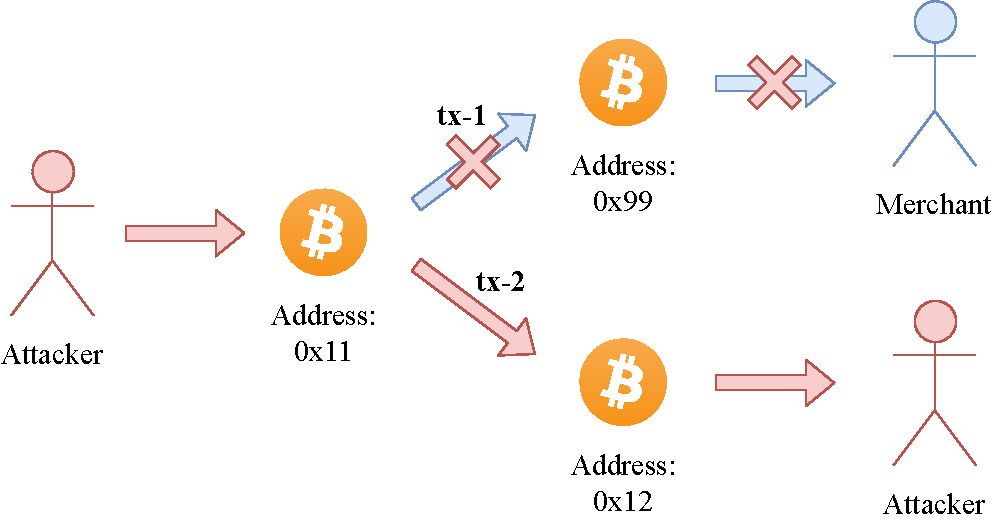
\includegraphics[scale=0.8]{figures/race_attack}
	\vspace*{0.25cm}
	\caption{
		Illustration of the race attack, a variant of double-spending.
		The attacker (in red) owns some bitcoins in the address \texttt{0x11}.
		It submits a transaction \texttt{tx-1} to move the money from its address \texttt{0x11} to the merchant's one \texttt{0x99}.
		At the same time, it submit to the Bitcoin network a conflicting transaction \texttt{tx-2} to move the the money from \texttt{0x11} to a new address \texttt{0x12} in its control.
		If the network includes \texttt{tx-2} in some block before \texttt{tx-1}, \texttt{tx-1} is rejected, and the money stay control of the attacker.
	}
	\label{fig:race-attack}
\end{figure}

A trivial way for the merchant to defend itself from this attack is to wait for the transaction \texttt{tx-1} to be stored in the blockchain:
if it is rejected because of any conflicts, the merchant can simply refuse the payment and do not sell the good.
Unfortunately, Bitcoin requires on average \SI{10}{minutes} to confirm a transaction, so this technique can not be applied to every case.

\section{Majority Attack}
51\%
\cite{selfish_mining, selfish_mining_acm}
